\section{Vue d'ensemble des groupes}Sur cette page, vous voyez vos groupes de postes client et le nombre de postes client y appartenants. Apr\`es un clic sur le nom d'un groupe, vous verrez la page avec les d\'etails sur le groupe respectif.\\
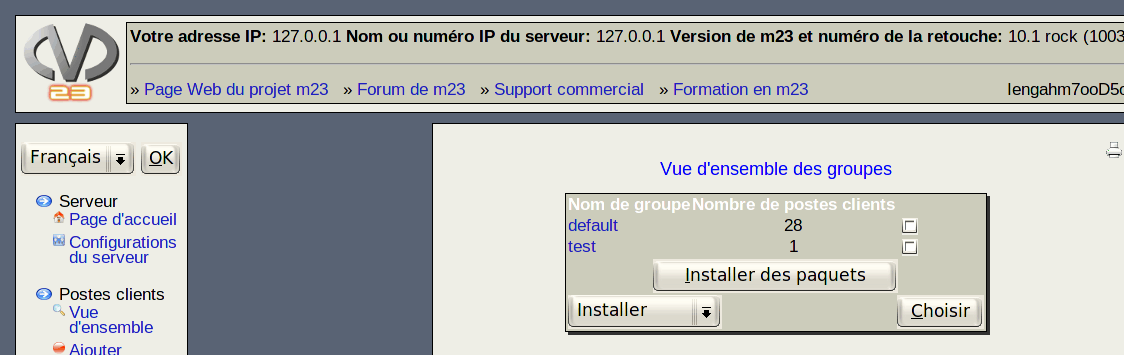
\includegraphics[scale=0.4]{/mdk/doc/manual/screenshots/fr/groups_overview.png} \\
\subsection{Donner des t\^aches \`a un groupe}
Vous pouvez donner des t\^aches aux postes client d'un ou de plusieurs groupes et, de cette fa\c{c}on, faciliter beaucoup l'administration durant l'installation, la d\'esinstallation ou la mise \`a jour.\\
\subsection{Proc\'edez comme c'est d\'ecrit au suivant:}
\begin{enumerate}
\item Choisissez l'action souhait\'ee de la liste.\\
\item Cliquez sur \textit{$\ll$Choisir$\gg$} et puis, le bouton d'action va afficher l'action choisie.\\
\item S\'electionnez le(s) groupe(s).\\
\item Enfin, double-cliquez sur le bouton d'action.\\
\end{enumerate}
